\mnAdvanced
\begin{slikaDesno}{fig/Q_u_C.pdf}
    \PID Математичко клатно, сачињено из мале  
    куглице, наелектрисања $Q = 1\unit{nC} $, и танке неистегљиве нити дужине ${L = 1\unit{m}}$, 
    постављено је у унутрашњост равног плочастог кондензатора растојања између облога 
    $d = 100\unit{mm}$. Једна облога кондензатора је на 
    референтном потенцијалу док се друга може помоћу преклопника $\Uppi$ пребацивати 
    између прикључка идеалног напонског генератора сталног напона $V_{\rm G} = 9\unit{kV}$ и 
    референтног потенцијала, као што је приказано на слици. 
    
\end{slikaDesno}
Сила отпора средине може се представити у облику ${\bf F}_{\rm ov} = - b {\bf v}$, где је $b = \dfrac{200}{3} \unit{\dfrac{\upmu N}{m/s}}$.
Гравитационо убрзање је $g = 9,81\unit{\dfrac{m}{s^2}}$ и оријентисано је као на слици. 
\begin{enumerate}[label=(\alph*)]
    \item Посматра се систем, чији је једини улаз напон кондензатора $u = u(t)$ а једини излаз отклон клатна 
    $\uptheta = \uptheta(t)$. Одредити функцију преноса тог система 
    $H(s) = \dfrac{\Uptheta(s)}{U(s)}$.
    \item До тренутка $t = 0$ прекидач $\Uppi$ је у стању (0). У тренутку $t = 0$ први пут мења стање, а затим  
    мења стање сваки пут у тренуцима $t = kT$, $k \in \mathbb N$, $f = \dfrac 1T$. Одредити израз за 
    $u(t)$. Пошто разматрани систем има релативно висок $Q$ фактор, уколико се разматра резонантна побуда, релевантан је 
    утицај само основног хармоника (на резонантној учестаности). Сигнал $u(t)$ развити у Фуријеов ред па 
    апроксимирати побудни напон основним хармоником $u(t) = U_{\rm m} \sin(\upomega t) \uu(t)$, а 
    на основу те апроксимације одредити $U(s)$. Сматрати да је $\upomega$ за 5\% веће од сопствене учестаности 
    клатна. 
    \item Полазећи од резултата претходних тачака, одредити израз за $\Uptheta(s)$ и одредити комплетан одзив 
    посматраног система. 
\end{enumerate}

\RESENJE
(а) Унутар кондензатора постоји хомогено електрично поље $E$, услед кога на куглицу 
делује електрична сила $F = QE$.
Једначина другог Њутновог закона за ротационо кретање клатна, у облику $J \dfrac{\de\uptheta}{\de t} = M$ за
куглицу онда гласи:
\begin{eqnarray} 
    mL^2 \dfrac{\de^2 \uptheta}{\de t^2} &=& - b L^2 \dfrac{\de \uptheta}{\de t} - mgL\sin(\uptheta) + QE L\cos(\uptheta) \Rightarrow \\[1mm]
    \dfrac{\de^2 \uptheta}{\de t^2} &=& - \dfrac{b}{m}  \dfrac{\de \uptheta}{\de t} - \dfrac{g}{L} \sin(\uptheta) + \dfrac{QE}{mL}\cos(\uptheta)
\end{eqnarray}
Уколико применимо апроксимацију малог угла $\sin\uptheta \approx \uptheta$, односно $\cos \uptheta \approx 1$, као и заменимо 
израз за јачину електричног поља у области кондензатора $U = \dfrac{E}{d}$, даље се Лапласовом трансформацијом налази 
\begin{eqnarray}
    \dfrac{\de^2 \uptheta}{\de t^2} + \dfrac{b}{m}  \dfrac{\de \uptheta}{\de t} + \dfrac{g}{L} \uptheta =  \dfrac{Q}{mdL} u
    \overset{{\LT{\bullet}}}{ \Rightarrow } 
    \left(
        s^2 + \dfrac{b}{m} s +  \dfrac{g}{L}
    \right) \Uptheta(s) 
    =
    \dfrac{Q}{mdL} U(s)
\end{eqnarray}
Одакле се непосредно налази:
\begin{eqnarray}
    H(s) = \dfrac{ H_0 }{s^2 + \dfrac{1}{\uptau} s + \upomega_{\rm k}^2}, \quad && H_0 = \dfrac{Q}{mdL} \approx 10^{-5} \unit{\dfrac{1}{Vs^2}} ,\, \uptau = \dfrac{m}{b} 
    \approx 15\unit{s},\,  \\
    && \upomega_{\rm k} = \sqrt{\dfrac{g}{L}} \approx 3,13\unit{\dfrac{rad}{s}}
\end{eqnarray}
Добијена квадратна форма може се средити допуњавањем до квадрата бинома као 
$ H(s) = s^2 + \dfrac{1}{\uptau} s + \upomega_{\rm k}^2 = s^2 + 2 \dfrac{1}{2\uptau} s + \dfrac{1}{4\uptau^2} + \upomega_{\rm k}^2 - \dfrac{1}{4\uptau^2} 
= \left( s + \dfrac{1}{2\uptau} \right)^2 +  \upomega_0^2 - \dfrac{1}{4\uptau^2}$, па се онда добијена функција преноса може изразити и као 
\begin{eqnarray}
    H(s) = \dfrac{H_0}{(s + \upsigma)^2 + \upomega_0^2}, \qquad \upsigma = \dfrac{1}{2\uptau} \approx \dfrac{1}{30} \unit{s^{-1}} \quad \upomega_0 = \sqrt{\upomega_{\rm k}^2 - \dfrac{1}{4\uptau^2} }
    \approx \upomega_k
\end{eqnarray}

(б) Дати сигнал се може записати у временском домену као 
$u(t) = V_{\rm G} \sum_{k = 0}^{\infty} \uu(t - kT) - \uu(t - (k+1/2)T)$, односно, представља униполарну правоугаону поворку 
правоугаоних импулса. 
На основу резултата задатка \ref{z:rect_povorka} је комплексни спектар разматраног сигнала
$U[k] = \dfrac{V_{\rm G}}{2} \sinc\left(\dfrac{k}{2}\right) \ee^{-\jj k \uppi / 2 } $.
На основу тога је
$U[1] = \dfrac{V_{\rm G}}{2} \dfrac{2}{\uppi} \ee^{-\jj\uppi/2} = - \jj \dfrac{V_{\rm G}}{\uppi}$.
Помоћу везе између развоја у тригонометријски и комплексан Фуријеов ред\footnote{Користи се 
резултат $X[k] = \dfrac{A[k] - \jj B[k]}{2} \Rightarrow B[k] = -2 \Im{X[k]}$.
}, онда се може писати, помоћу табличне трансформације \reft{T:LT:sin}, да је 
\begin{equation}
    u(t) \approx \dfrac{V_{\rm G}}{2}  
    \dfrac{4}{\uppi} \sin(\upomega t) .
    \Rightarrow
    U(s) = 
    \dfrac{2 V_{\rm G}}{\uppi}
    \dfrac{\upomega }{s^2 + \upomega^2}
\end{equation}

(в) Помоћу резултата претходних тачака, Лапласова трансформација одзива дата је у облику: 
\begin{equation}
    \Uptheta(s) =
    \dfrac{H_0}{(s + \upsigma)^2 + \upomega_0^2}
    \cdot
    \dfrac{2 V_{\rm G}}{\uppi}
    \dfrac{\upomega_0 }{s^2 + \upomega_0^2}
    = 
    \dfrac{2 H_0 V_{\rm G}}{\uppi}
    \dfrac{1}{(s + \upsigma)^2 + \upomega_0^2}
    \cdot
    \dfrac{\upomega }{s^2 + \upomega^2}
\end{equation}
Инверзна Лапласова трансформација обавља се растављањем на парцијалне разломке, чиме се добија 
\begin{equation}
    H(s) = 
    \dfrac{2 H_0 V_{\rm G}}{\uppi} \left(
    \dfrac{A}{ s - (\upsigma + \jj\upomega_0 ) } + \dfrac{A^\ast}{ s - (\upsigma - \jj\upomega_0 ) } 
    + \dfrac{B}{s - \jj\upomega} + \dfrac{B^*}{s + \jj\upomega}  
    \right)
\end{equation}
Коефицијенти се налазе поступком који је детаљно описан у додатку \ref{a:pfd}, чиме се добијају
\begin{eqnarray}
    A &=& \dfrac{1}{\jj2\upomega_0} \dfrac{\upomega^2}{ \underbrace{( \upsigma + \jj\upomega_0)^2}_{\upsigma \ll \upomega_0} + \upomega^2 }
   \approx 
   - \jj
   \dfrac{1}{2} \dfrac{\upomega/\upomega_0} { \upomega^2 - \upomega_0^2 } \\
   B &=& \dfrac{1}{ (\jj\upomega + \upsigma)^2 + \upomega_0^2 } \dfrac{\upomega}{\jj2\upomega}
   \approx
   - \jj 
   \dfrac{1}{2} 
   \dfrac{1}{\upomega_0^2 - \upomega^2}
\end{eqnarray},
Одавде се коначно, на основу резултата задатка \ref{z:damp_sin} има 
\begin{equation}
    \uptheta(t) = \dfrac{2 H_0 V_{\rm g}}{\uppi}
    \dfrac{1}{\upomega_0^2 - \upomega^2}
    \left(
        \sin(\upomega t )
        -
        \dfrac{\upomega}{\upomega_0} \ee^{-\upsigma t} \sin(\upomega_0 t ). \label{\ID.odziv}
    \right)
\end{equation}

Ради бољег квалитативног описа добијеног резултата, по узору на поступак из задатка \ref{z:LC_izbijanje}, усвојићемо  
да је побудна учестаност у околини резонантне учестаности клатна 
$\upomega_0 = \upomega + \Updelta\upomega$, $\Delta \upomega \ll \upomega$. Одатле се може писати да је\footnote{
    Користи се Бернулијева апроксимација $(1+x)^\upalpha \approx 1 + \upalpha x$, $x \ll 1$; као и формула за синус збира
    $\sin(x+y) = \sin(x)\cos(y) + \cos(y)\sin(y)$
}
$
\dfrac{\upomega}{\upomega_0} = \dfrac{\upomega}{\upomega + \Delta \upomega} = \left(1 + \dfrac{\Delta \upomega}{\upomega} \right)^{-1} \approx 
1 - \dfrac{\Delta \upomega}{\upomega}$; као и 
$
\dfrac{1}{\upomega_0^2 - \upomega^2} = 
\dfrac{1}{\underbrace{(\upomega_0 - \upomega)}_{\Delta\upomega} \underbrace{(\upomega_0 + \upomega)}_{\approx 2\upomega} } \approx 
\dfrac{1}{2\upomega \Delta \upomega}
$, па се заменом у \eqref{\ID.odziv} налази 
\begin{eqnarray*}
    && \uptheta(t) \approx \dfrac{H_0 V_{\rm g}}{\uppi \upomega \Delta \upomega}
    \left(
        \sin(\upomega t )
        -
        \left(1 - \dfrac{\Delta \upomega}{\upomega}\right) \ee^{-\upsigma t} \sin( (\upomega + \Delta \upomega) t )
    \right) \\
    &&=
    \dfrac{H_0 V_{\rm g}}{\uppi \upomega \Delta \upomega}
    \left(
        \sin(\upomega t )
        -
        \left(1 - \dfrac{\Delta \upomega}{\upomega}\right) \ee^{-\upsigma t} 
        \left(
            \sin( \upomega t )  \cos(\Delta \upomega t ) + \cos( \upomega t )  \underbrace{\sin(\Delta \upomega t ) }_{\approx 0}
        \right)
    \right) \\ 
    && \approx
    \underbrace{\dfrac{H_0 V_{\rm g}}{\uppi \upomega \Delta \upomega}
        \left(
            1 - \left(1 - \dfrac{\Delta \upomega}{\upomega}\right) \ee^{-\upsigma t} \cos(\Delta \upomega t ) 
        \right)}_{A(t)} \sin(\upomega t),
\end{eqnarray*}
којом приликом је члан са $\sin(\Delta\upomega t)$ занемарен јер он брзо ишчезава са временом, а током времена током ког је члан релевантан, 
је његова амплитуда мала јер је тада $\Delta \upomega t \ll 1$. Добијени сигнал представља простопериодични сигнал променљиве амплитуде 
$A \approx A(t)$ 
који сам представља пригушену синусоиду учестаности која одговара разлици $\Delta \upomega$. Резултат је приказан на слици \ref{\ID.res}, 
на којој је и уцртан и апроксимативни сигнал анвелопе $A(t)$.

\begin{figure}[ht!]
    \centering
    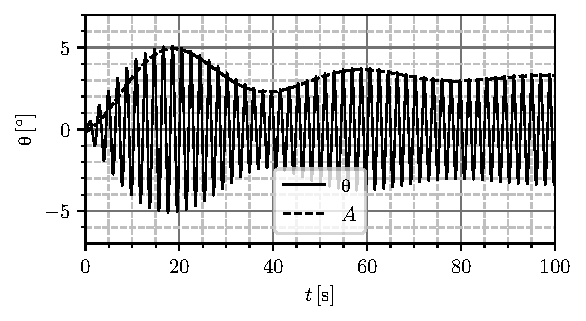
\includegraphics{fig/klatno_plot.pdf}
    \caption{Временски дијаграм одзива клатна, за $\Updelta \upomega \approx 5\% \upomega_0$}
    \label{\ID.res}
\end{figure}